\documentclass{article}[12pt]
\usepackage{listings}
\usepackage{color}
\usepackage{amsmath}
\usepackage{graphicx}
\usepackage{float}
\usepackage{amssymb}
\usepackage{mathtools,amssymb}
\usepackage{amsfonts}
\usepackage{amsthm}
\usepackage[linguistics]{forest}
\usepackage[utf8]{inputenc} 
\usepackage{chngcntr}
\usepackage{subcaption}
\usepackage[top=2in, bottom=1.5in, left=1in, right=1in]{geometry}
\usepackage{graphicx}
\usepackage{amsfonts}
\usepackage{amssymb}
\usepackage{amsmath}
\usepackage{setspace}
\setstretch{1,4}
\usepackage[francais]{babel}
\usetikzlibrary{quotes,arrows.meta}
\tikzset{
  annotated cuboid/.pic={
    \tikzset{%
      every edge quotes/.append style={midway, auto},
      /cuboid/.cd,
      #1
    }
    \draw [every edge/.append style={pic actions, densely dashed, opacity=0.5}, pic actions]
    (0,0,0) coordinate (o) -- ++(-\cubescale*\cubex,0,0) coordinate (a) -- ++(0,-\cubescale*\cubey,0) coordinate (b) edge coordinate [pos=1] (g) ++(0,0,-\cubescale*\cubez)  -- ++(\cubescale*\cubex,0,0) coordinate (c) -- cycle
    (o) -- ++(0,0,-\cubescale*\cubez) coordinate (d) -- ++(0,-\cubescale*\cubey,0) coordinate (e) edge (g) -- (c) -- cycle
    (o) -- (a) -- ++(0,0,-\cubescale*\cubez) coordinate (f) edge (g) -- (d) -- cycle;
    \path [every edge/.append style={pic actions, |-|}]
    (b) +(0,-5pt) coordinate (b1) edge ["\cubex \cubeunits"'] (b1 -| c)
    (b) +(-5pt,0) coordinate (b2) edge ["\cubey \cubeunits"] (b2 |- a)
    (c) +(3.5pt,-3.5pt) coordinate (c2) edge ["\cubez \cubeunits"'] ([xshift=3.5pt,yshift=-3.5pt]e)
    ;
  },
  /cuboid/.search also={/tikz},
  /cuboid/.cd,
  width/.store in=\cubex,
  height/.store in=\cubey,
  depth/.store in=\cubez,
  units/.store in=\cubeunits,
  scale/.store in=\cubescale,
  width=10,
  height=10,
  depth=10,
  units=cm,
  scale=.1,
}

\newcommand{\R}{\mathbb{R}}

\newcommand{\change}{\textcolor{blue}}
\newcommand{\argmin}{\mathop{\mathrm{arg\,min}}}
\newcommand{\argmax}{\mathop{\mathrm{arg\,max}}} 

\counterwithin*{section}{part}
\definecolor{mGreen}{rgb}{0,0.6,0}
\definecolor{mGray}{rgb}{0.5,0.5,0.5}
\definecolor{mPurple}{rgb}{0.58,0,0.82}
\definecolor{backgroundColour}{rgb}{0.95,0.95,0.92}
\lstdefinestyle{CStyle}{
    backgroundcolor=\color{backgroundColour},   
    commentstyle=\color{mGreen},
    keywordstyle=\color{magenta},
    numberstyle=\tiny\color{mGray},
    stringstyle=\color{mPurple},
    basicstyle=\footnotesize,
    breakatwhitespace=false,         
    breaklines=true,                 
    captionpos=b,                    
    keepspaces=true,                 
    numbers=left,                    
    numbersep=5pt,                  
    showspaces=false,                
    showstringspaces=false,
    showtabs=false,                  
    tabsize=2,
    language=C
}

\title{PLDAC - Etude de différentes techniques pour la classification de signaux d'EEG et MEG}
\author{Buton Nicolas, encadré par Vincent Guigue et Olivier Schwander}
\renewcommand{\contentsname}{Table des matières}
\begin{document}
\pagenumbering{gobble}
\maketitle
\begin{center}

\includegraphics[scale=1]{images/logoSorbonne.jpg}
\end{center}
\newpage
\tableofcontents
\newpage
\pagenumbering{arabic}
\part{Introduction}
Les signaux étudiés seront des signaux d'Électroencéphalographie(EEG) et de Magnétoencéphalographie(MEG). Le premier consiste à enregistrer les signaux électriques à la surface du crane grâce a des électrodes, le second enregistre l'activité magnétique induite par l'activité des neurones grâce a un ensemble de magnétomètres. Notre étude ce place dans le cadre de l'analyse de série temporelle multivariée. On retrouve ces séries dans plusieurs domaines comme en finance, géophysique et dans notre cas dans les BCI (Brain Computer Interface). Chaque variable possède une dimension temporelle et de plus chaque variable est liée spatialement aux autres.\\

Une des premières difficultés des interfaces cerveaux machines c'est qu'elles ont besoin de réagir vite cela implique que l'on doit analyser le signal sur un laps de temps court, ce qui nous donne peu de données pour voir les liens entre les différentes variables. Le fait que les électrodes ne sont jamais situées exactement au même endroit sur le crane entre chaque essai et entre chaque personne rajoute une autre difficulté. De plus il peut y avoir beaucoup de bruits générés par le matériel et les mouvements de l'utilisateur par exemple.\\

Historiquement la classification sur de tels signaux se faisait avec des méthodes linéaires, par exemple avec des SVM ou des régressions logistiques \cite{garcia_support_2003}. Cela avait des performances assez faible et il fallait donc répéter l’expérience plusieurs fois. Par la suite Alexandre Barachant a proposé d'utiliser les méthodes riemanniennes \cite{congedo_riemannian_2017}, celles-ci permettent de prendre en compte la spatialité des données et sont plus robustes. Cette robustesse vient du fait que la géométrie de Riemann permet de manipuler des matrices de covariance. On peut définir une distance entre matrices symétriques définies positives et les matrices de covariance font partie de ce groupe. Ces méthodes ont permis d'attaquer des taches plus compliqués comme le transfert entre participants. On entraîne notre modèle en utilisant un participant pour faire ensuite des prédictions sur un autre participant.\\

C'est pour cela qu'aujourd'hui dans les méthodes de l’état de l'art on utilise encore la géométrie riemannienne. Par la suite nous allons comparer ces méthodes avec de la géométrie riemannienne avec d'autres méthodes plus classiques, ainsi qu'une méthode de deep learning (un réseaux convolutionel). Nous essayerons plusieurs combinaisons avec des méthodes issues du traitement du signal comme la transformée de Fourier, des filtres et aussi d'autre façon de traiter les matrices de covariance avec des modèles comme des SVM ou KNN. Par ailleurs nous étudierons aussi l'effet de la taille de la fenêtre.\\

On pourra voir que pour des cas simples comme l'ouverture et la fermeture des yeux qui possèdent un signal très fort sur un EEG on a déjà de très bon résultats avec des méthodes simples, F1-score de 0.77 sur la classe minoritaire avec une transformée de Fourier puis un SVM avec une taille de fenêtre adaptée (plus de détails dans la partie expérimentation), et avec un "Minimum distance to Mean" et de la géométrie riemannienne on obtient un F1-score de 0.84.\\

\part{État de l'art - la géométrie de Riemann}
Nous avons besoins de métrique dans des espaces de Riemann pour pouvoir comparer les matrices entre elles. Cela nous permet de transposer des algorithmes comme les plus proches voisins ou les MDM, ou l'on définit un centre par classe et on regarde de quel centre est plus proche la nouvelle données. Et nous avons aussi besoin d'un façon de vectorisé cette matrice et c'est a cela que sert l'espace tangent.


\section{Espace tangent}
Pour avoir un variété riemannien il nous faut un espace tangent. Et pour avoir un espace tangent il nous faut une distance locale. De plus on sait que l'espace des paramètre des gaussiennes multivariées possèdent un produit scalaire local(obtenu par différentiation), donc une distance locale. Un des paramètre de cette gaussienne étant une matrice de covariance, cela nous définit donc une variété riemannienne sur les matrices SDP(symétriques définies positives). Car une matrice SDP quelconque  peut être vu comme une matrice de covariance.

L'espace tangent est un espace euclidien. On peut approximer des distances de l'espace de Riemann par des distances dans l'espace tangent et cela fonctionne assez bien localement. On peut projeter un point de l'espace de Riemann définit par une matrice $N*N$ sur un espace tangent avec $N(N+1)/2$ dimensions. Pour cela il faut choisir un point pour définir notre espace tangent. Autour de ce point on aura une très bonne estimation de la distance et plus on s'en éloigne et plus l'estimation sera mauvaise. Mais il a été remarqué qu’expérimentalement pour de la classification le point que l'on choisi change peu le résultat. C'est pour cela que par la suite nous prendrons l'identité(qui est une matrice SDP) comme point pour définir notre espace tangent.

\begin{figure}[H]
\begin{center}
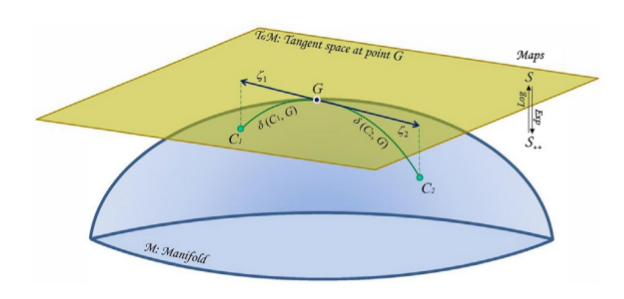
\includegraphics[scale=0.5]{images/Riemann_tangent_space.png}
\end{center}
\caption{Affichage de l'espace tangent}
\end{figure}


\section{Distance globale}
La distance géodésique est la longueur du plus court chemin entre deux point sur la variété. On peut calculer cette distance par morceau en faisant des petit pas et avec la distance locale, mais de la cas générale on n'a pas de formule. Par contre dans le cas des matrices symétriques et définies positives on a la formule qui est la suivante :

Soit deux matrices $\mathbf{\Sigma}_1$ et $\mathbf{\Sigma}_2$ symétriques et définies positives.
\begin{equation}
\label{eq:Rgeodistance}
\delta_R(\mathbf{\Sigma}_1,\mathbf{\Sigma}_2) 
= 
\Vert \mathrm{log} \left( \mathbf{\Sigma}_1^{-1/2} \mathbf{\Sigma}_2 \mathbf{\Sigma}_1^{-1/2} \right) \Vert_F
=
\left[ \sum_{c=1}^{C} \log^2 \lambda_c \right]^{1/2},
\end{equation}
où $\lambda_c, c=1\ldots C$ sont les valeurs propres réelles de $\mathbf{\Sigma}_1^{-1/2} \mathbf{\Sigma}_2 \mathbf{\Sigma}_1^{-1/2}$ et C le nombre d’électrodes.
\\
F : Norme de Frobenius

\section{Barycentre riemannien}
La définition du barycentre est :
\begin{equation}
\mathfrak{G} \left( \mathbf{\Sigma}_1,\ldots,\mathbf{\Sigma}_I \right) = \argmin_{\mathbf{\Sigma}} 
\sum_{i=1}^{I} 
\delta_R^2 \left( \mathbf{\Sigma},\mathbf{\Sigma}_i \right).
\label{eq:geo_mean}
\end{equation}
Malheureusement contrairement au cas euclidien ce n'est pas la même formule que la moyenne arithmétique. Et même restreins aux matrices SDP nous ne possédons pas d'expression explicite. Nous devons donc utiliser un algorithme itératif. Nous définissons donc une matrice $\mathbf{\Sigma}_i$, matrice moyenne que nous initialisons aléatoirement et ensuite on procède par descente de gradient pour approximer le barycentre.\\
\\
Pour plus de détails sur la géometrie de riemann il y a cet article d'A. Barachant \cite{congedo_riemannian_2017}.
\part{Plan d'expérience}
\section{Arbre des modèles}
Nous allons représenter à l'aide d'un arbre les différentes méthodes que nous allons tester par la suite.
\begin{center}
\begin{forest}
[Signal brut
  [Filtre passe-bas
	[SVM(8)]  
	[KNN(9)]
  ]
  [TF
  	[SVM(1)]
  	[KNN(2)]
  ]
  [Cov
  	[SVM(3)]
  	[MDM(4)]
  	[KNN(5)]
  ]
  [SVM(6)]
  [KNN(7)]
  [CTR(8)]
]
\end{forest}
\end{center}

Légende :\\
Cov : Matrice de covariance\\
TF : Transformée de Fourier\\
MDM : Minimum Distance to Mean\\
CTR : Chaîne de traitement riemannienne, détaillée plus loin.
\\

\section{Format des données}
En entrée deux formats sont possible. Le premier est une série temporelle pour chaque électrodes ainsi que les labels pour chaque donnée d'entrée.\\
Notons :\\
C : le nombre de canaux.\\
T : le temps écoulé en seconde pendant l'enregistrement des données.\\
f : la fréquence d’échantillonnage du signal.\\
$D_{E}$ : durée d'un essai.\\
$N_{T}$ : le nombre de trial.\\
Nous disposons donc d'une matrice de taille $C*(T*f)$, ainsi que d'un vecteur de label de taille $(T*f)$.\\
\\
Mais un deuxième format d'entré est possible, en découpant par trial, a chaque trial correspond un label. Nous disposons donc d'un tenseur de taille $(D_{E}*f)*C*N_{T}$, et d'un vecteur de label de taille $N_{T}$.\\
On peut passer du premier formalisme a l'autre en découpant par trial (en définissant une taille de fenêtre) mais nous avons plusieurs possibilités pour savoir quel label associé à ce trial (label majoritaire,premier label,dernier label,etc...).\\
\section{Description des modèles}
Une donnée correspond à un essai. On le note $x\in \mathbb{R}^{C*D_{E}}$. Si les signaux sont présentés en continu il faut les découper en choisissant une taille de fenêtre pour les analysés.
\paragraph{1 et 2 - SVM et KNN avec une transformée de Fourier}\mbox{}\\
La première étape de notre modèle est d'effectuer une transformée de Fourier, c'est a dire passer d'un signal temporel à un signal fréquentiel. Pour calculer cette transformation nous utiliserons l'algorithme FFT (Fast Fourier transform). Nous garderons uniquement le module pour rester avec des valeurs réelles plutôt que complexes. Ensuite nous utilisons un SVM linéaire pour prédire les labels dans un cas et un KNN euclidien dans l'autre. Les données apres pré-traitement $x_{fft}\in \mathbb{R}^{C*\left\lfloor\dfrac{D_{E}}{2}\right\rfloor}$
\paragraph{3,4 et 5 - SVM,MDM et KNN avec matrice de covariance }
\mbox{}\\
Pour cette approche nous devons passer au deuxième format de données. On calcule la matrice de covariance.$\Sigma=x^T*x\in \mathbb{R}^{C*C}$. Ces représentation sont reconnues très efficaces dans l'approche Riemannien. Nous allons vérifier ce que ça donne avec des approches plus classiques.
\paragraph{6 et 7 - SVM et KNN sur les données brutes}\mbox{}\\
Cette approche est la plus simple et on utilise simplement un vecteur de la taille le nombre de capteur, c'est à dire un relevé a un instant t des capteurs pour prédire un labels.
\paragraph{8 et 9 - SVM et KNN avec un filtre passe bas}\mbox{}\\
Nous définissons un filtre passe bas avec la moyenne sur un fenêtre glissante. Donc nous avons deux paramètres le premier est la longueur de la fenêtre, sur combien on moyenne et le deuxième est le décalage de cette fenêtre. On peut mettre la longueur de la fenêtre égale au décalage si on ne veux pas de chevauchement.
\paragraph{8 - Chaîne de traitement riemannienne}\mbox{}\\
Par la suite je vais décrire la chaîne de traitement étape par étape. Cette chaîne de traitement est spécifique au dataset DecMeg2014.\\
1 - On garde uniquement 1 seconde sur les 1.5 seconde de signal car le stimulus intervient qu’après 0.5 seconde. \\
2 - On filtre le signal avec un filtre passe bande de Butterworth d'ordre 5 entre 1Hz et 20Hz.\\
3 - Par la suite on effectue un filtrage spatial, on extrait $C_{virt}$ canaux virtuels par classe et K le nombre de classes \cite{rivet_xdawn_2009}. On commence par définir la moyenne sur chaque classe :
$$ \mbox{\Large $ 
\mathbf{P}^{(k)}=\frac{1}{ | \mathcal{I}^{(k) |}} \sum_{i \in \mathcal{I}^{(k)}} \mathbf{X}_{i_{1}}
$ } $$
Ensuite notre but est d'optimiser w par descente de gradient. En minimisant cette fonction :
$$ \mbox{\Large $ 
f(X,w)=- \frac{\mathbf{w}^{T} \mathbf{P}^{(k)} \mathbf{P}^{(k) T} \mathbf{w}}{\mathbf{w}^{T} \mathbf{X} \mathbf{X}^{T} \mathbf{w}}
$ } $$
On introduit les Zi :
$$ \mbox{\Large $ 
\mathbf{Z}_{i}=\mathbf{W}^{T} \mathbf{X}_{i}
$ } $$
4 - On définit une nouvelle entrée comme étant la concaténation :\\
- du signal moyen de la classe 1 auquel on multiplie par $W_{0}$ pour les projeter sur les canaux virtuels appris précédemment.\\
- idem pour la classe 2\\
- Et ensuite le signal $X_{i}$ projeté sur les 8 canaux, qui est $Z_{i}$.\\
Cela nous permet de définir de nouvelles caractéristiques, donc a chaque Xi d'entrée sur C canaux on le projette sur Cvirt canaux.
$$ \mbox{\Large $ 
\tilde{\boldsymbol{Z}}_{i}=\left[ \begin{array}{c}{\mathbf{W}^{(0)^{T}} \mathbf{P}^{(0)}} \\ {\mathbf{W}^{(1)^{T}} \mathbf{P}^{(1)}} \\ {\mathbf{Z}_{i}}\end{array}\right]
$ } $$
5 - On calcule la covariance spatiale de cette nouvelle matrice de caractéristique.
$$ \mbox{\Large $ 
\boldsymbol{\Sigma}_{i}=\frac{1}{N} \tilde{\mathbf{Z}}_{i} \tilde{\mathbf{Z}}_{i}^{T}
$ } $$
6 - On projette cette matrice sur l'espace tangent.\\
7 - On estime pour les 15 autres participants avec ce filtre spatial\\
8 - On fait la même chose pour les 15 autres participants et on concatène.\\
9 - On fait une régression logistique avec une régularisation lasso.\\
La figure suivante (Figure 2) représente la forme des matrices au fur et à mesure du processus. Les tailles des matrices correspondent aux tailles dans le dataset DecMeg2014. Elles sont à lire de gauche à droite et de haut en bas.
\\
\begin{figure}[H]
\label{fig2}
\begin{tikzpicture}
  \pic at (0,10) {annotated cuboid={width=375, height=306, depth=580, scale=.01, units=}};
  \pic at (5,10) {annotated cuboid={width=250, height=306, depth=580, scale=.01, units=}};
   \pic at (-4,4) {annotated cuboid={width=125, height=16, depth=580, scale=.01, units=}};
   \pic at (-2,4) {annotated cuboid={width=16, height=16, depth=580, scale=.01, units=}};
   \pic at (1,4) {annotated cuboid={width=136, height=1, depth=580, scale=.01, units=}};
   \pic at (3,4) {annotated cuboid={width=136, height=1, depth=9414, scale=.001, units=}};
   \pic at (-4,-1) {annotated cuboid={width=2176, height=1, depth=9414, scale=.001, units=}};
\end{tikzpicture}
\caption{Représentation des matrices au fur et à mesure des différentes étapes}
\end{figure}

\part{Experimentations}
Nous allons étudier nos méthodes sur 3 datasets différents : Eye close/eye open, brain invader et DecMeg2014. Dans un premier temps nous regarderons la valeur de K optimale pour les différents KNN, par la suite nous nous intéresserons à la taille de la fenêtre optimale, puis pour finir quelles méthodes fonctionnent le mieux selon la situation. Tout le code et les résultats correspondant aux expériences peuvent être trouvés sur github. \footnote{https://github.com/rootNico/PLDAC}
\section{Description des différents datasets}
\subsection{Description du dataset eye close/eye open}
Le dataset eye close/eye open contient les données enregistrées avec un casque EEG où l'on a demandé aux participants d'ouvrir ou de fermer les yeux à certains moments. La tâche à accomplir est de classifier à chaque enregistrement si la personne a les yeux ouverts ou fermés.\\
\\
Le signal est échantillonné à 512Hz. Il y a 7 femmes et 13 hommes pour un total de 20 participants pour ce dataset. L'age moyen est de 25.8 ans avec un écart type de 5.27 et une médiane de 25.5 ans. 18 participants ont entre 19 et 28 ans et deux participants ont respectivement 33 ans et 44 ans. Le casque d'enregistrement est composé de 16 électrodes.\\
\\
On commence par visualiser le signal des 16 électrodes ainsi que les labels associés au cours du temps. On peut voir que cette tâche, même si c'est une tâche relativement facile pour une machine, reste très difficile voir impossible pour un humain.\\
\begin{figure}[H]
\begin{center}
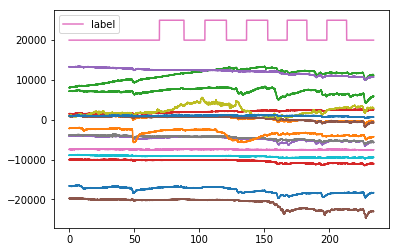
\includegraphics[scale=0.8]{images/donnees_entree.png}
\end{center}
\caption{Affichage des données brutes}
\end{figure}

\subsection{Description du dataset brain invader}
Il y a 24 participants qui ont participé à l’éxperience (12 femmes), avec une moyenne d'age (écart type) de 25.96 (4.46). Les 12 électrodes en vert sur l'image ci-dessous était utilisé.
\begin{figure}[H]
\begin{center}
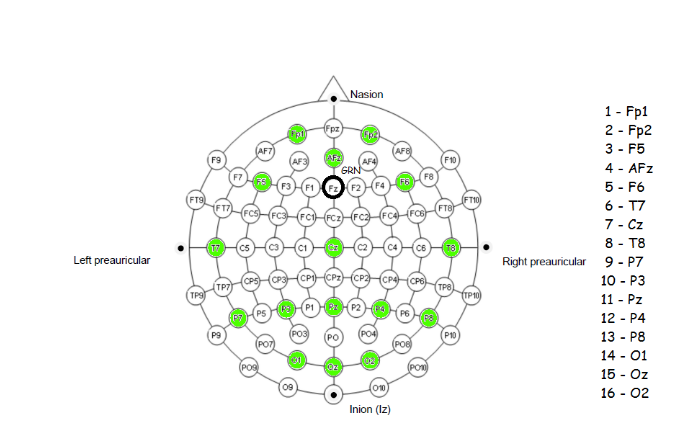
\includegraphics[scale=0.4]{images/situation_capteur.png}
\end{center}
\caption{Affichage des données brutes}
\end{figure}

Ce dataset a été enregistré avec les participants placés devant un pc ou une grille d'alien était représenté sur un écran avec un alien en particulier qui était en rouge. Le but pour le participant est de viser l'alien rouge. Pour cela 12 flashs dont 2 comprennent l'alien ciblé sont émis, le but de l'algorithme est de voir par quel flash le participant est intéressé. Un flash est composé de 
6 alien. En tout il y avait 36 aliens sur l’écran, une grille de 6X6. Il y a plusieurs tentatives pour détruire l'alien.\\
Les deux tâches suivantes sont à effectuer :\\
Première tache : Classification binaire (le flash nous intéresse, s'il y a l'alien cible dedans)\\
Deuxième tache : Il nous faut trouver les deux flashs comprenant l'alien ciblé dans le groupe des 12 flashs.\\
Mais comme nous allons le voir dans la partie résultat nous n'avons pas toute les informations pour traiter la deuxième tache.

Plusieurs datasets utilisent ce paradigme de P300. On présente un stimulus à un participant et environ 300 ms après on peut détecter une activité cérébrale. En répétant plusieurs fois l'opération, cela permet a l'utilisateur de faire un choix par la pensée.\\

\begin{figure*}[]
	\centering
    \begin{subfigure}[]{0.475\textwidth}
    	\centering
        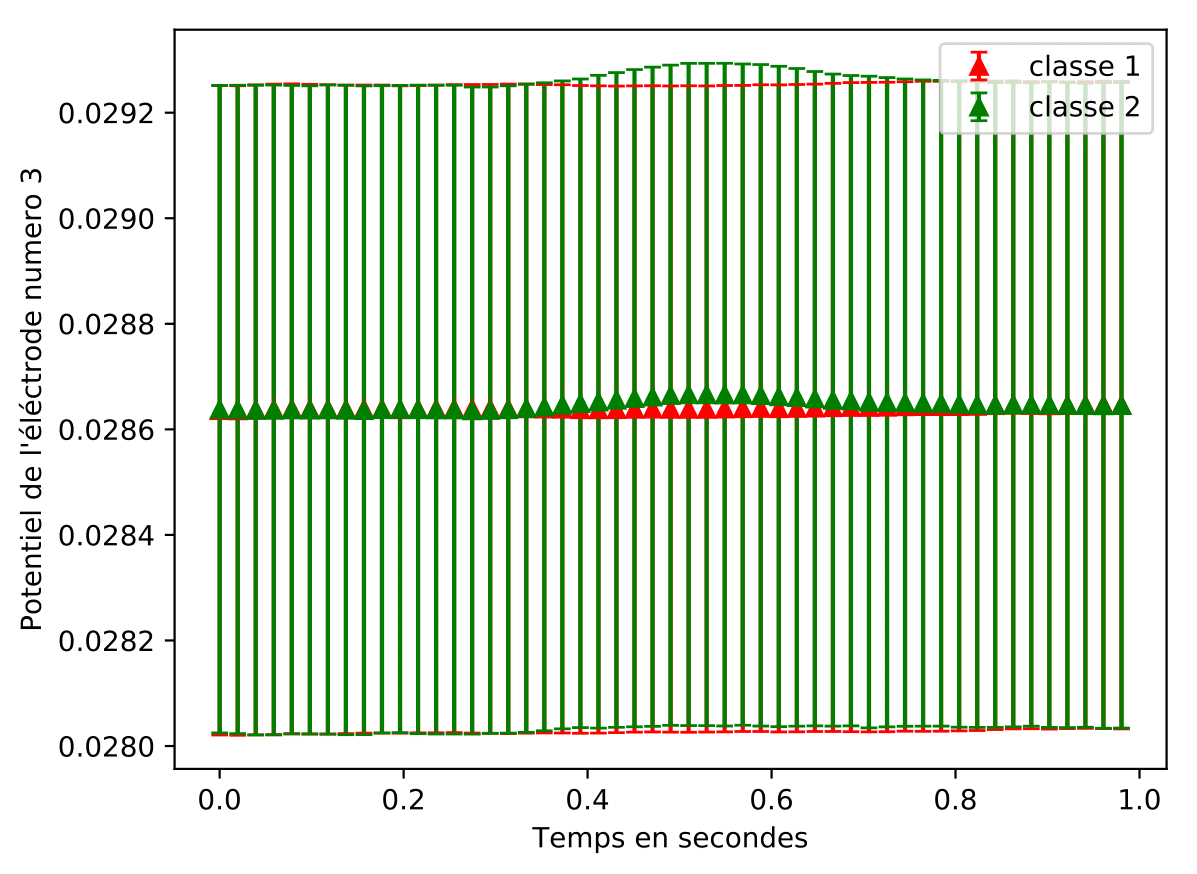
\includegraphics[width=\textwidth]{images/visuel_classe_mean_std-1.png}
        \caption[Network2]%
            {{\small visuel classe mean std}}    
        \label{fig:mean and std of net14}
	\end{subfigure}
    \hfill
    \begin{subfigure}[]{0.475\textwidth}  
     	\centering 
        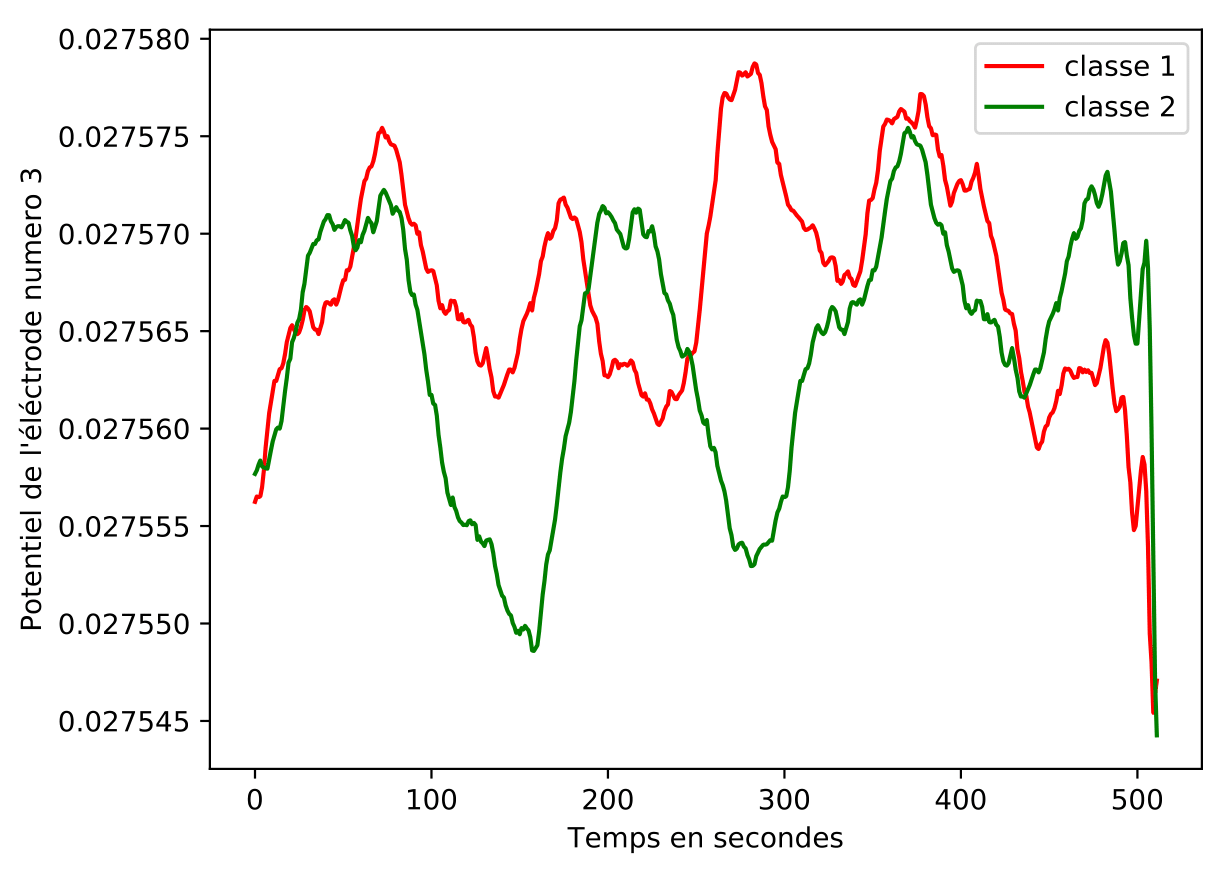
\includegraphics[width=\textwidth]{images/visuel_data_0-1.png}
        \caption[]%
            {{\small visuel data 0-1 }}    
        \label{fig:mean and std of net24}
    \end{subfigure}
    \caption[ Visualisation des classes]
        {\small Visualisation des classes} 
    \label{fig:mean and std of nets}
\end{figure*}
    
    
Figure 4 : Par la suite on peut voir sur l'image de droite le potentiel de l’électrode numéro 3 selon la classe au cours du temps. Et pour se rendre un peu mieux compte de la difficulté de la tâche on peut voir sur le graphique de gauche la moyenne sur tous les essais avec l’écart type, on peut différencier les deux classes mais l’écart entre les moyennes est très petit en comparaison des grandes valeurs des écarts types. Les graphiques sur les autres électrodes montrent tous à peu prêt la même chose ou parfois même encore moins d’écart de moyenne entre les deux classes.

\subsection{Description du dataset DecMeg2014}
La tâche que l'on doit réaliser avec le dataset DecMeg2014 est une classification binaire. Le but est de déterminer si le stimulus visuel est un visage clair ou brouillé qui est montré au participant. L'activité de leurs cerveaux est enregistré grâce à un appareil de magnetoencéphalographie. Cet appareil dispose de 306 magnétomètres.
\\
Ce dataset est extrait d'une compétition kaggle du même nom.
\\
Il y a eu 23 participants à ce test avec environ 580 essais par participant. Nous disposons de 16 participants avec leurs labels associé et 7 participants où nous avons uniquement les données.
\begin{figure}[H]
\begin{center}
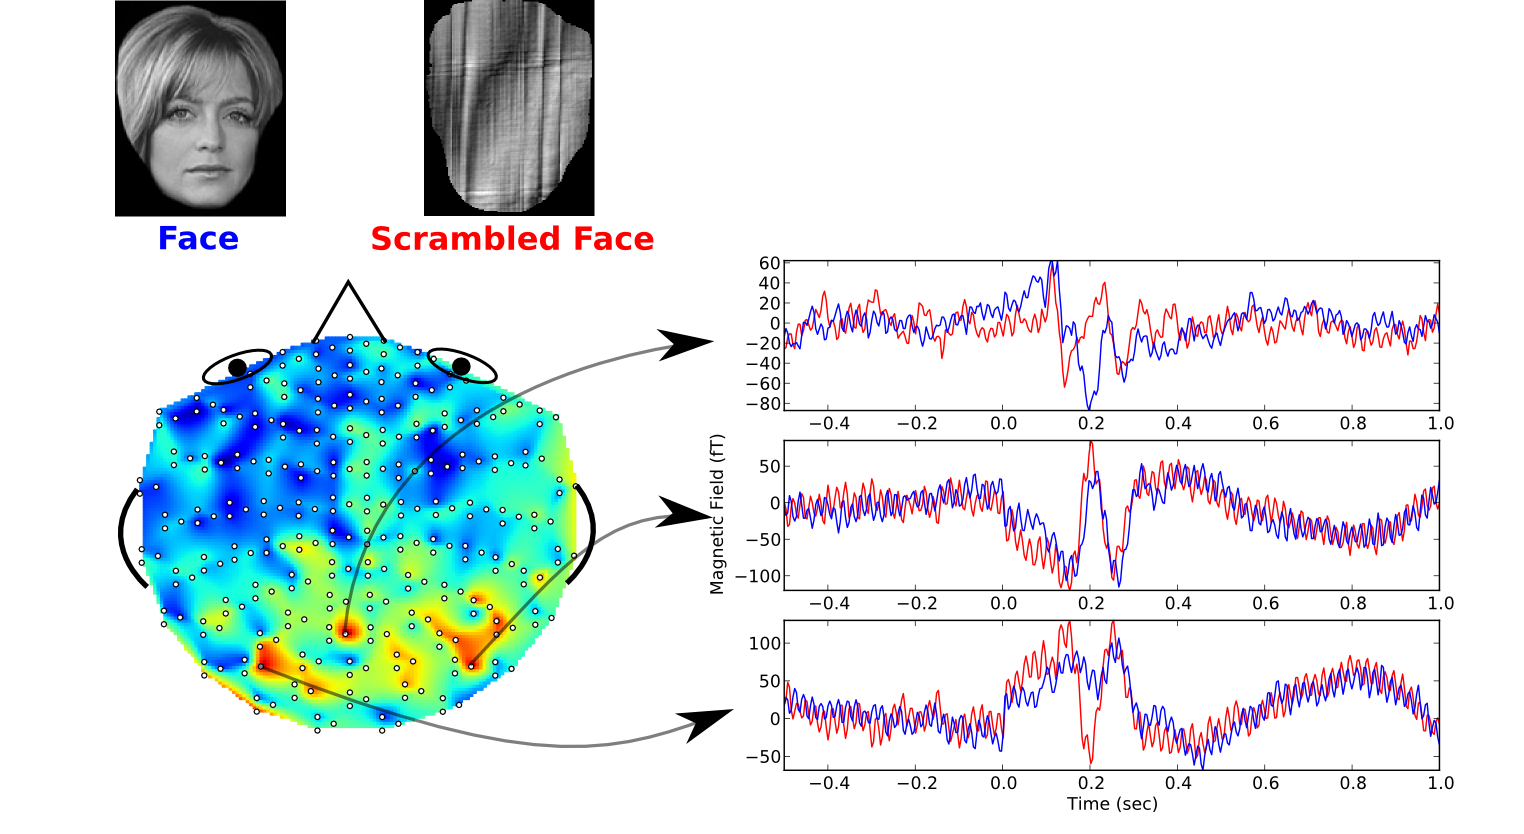
\includegraphics[scale=0.4]{images/DECMEG2014.png}
\end{center}
\caption{Taches DecMeg2014}
\end{figure}


\section{Étude sur les valeurs de k pour les différents KNN}

\begin{figure*}[h]
        \centering
        \begin{subfigure}[b]{0.475\textwidth}
            \centering
            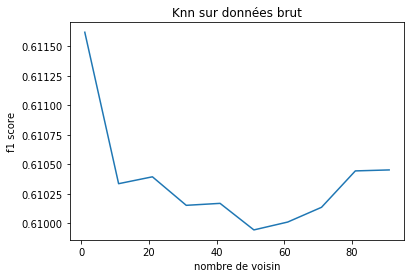
\includegraphics[width=\textwidth]{images/f1_score_knn_brut.png}
            \caption[Network2]%
            {{\small  knn sur les données brutese}}    
            \label{fig:mean and std of net14}
        \end{subfigure}
        \hfill
        \begin{subfigure}[b]{0.475\textwidth}  
            \centering 
            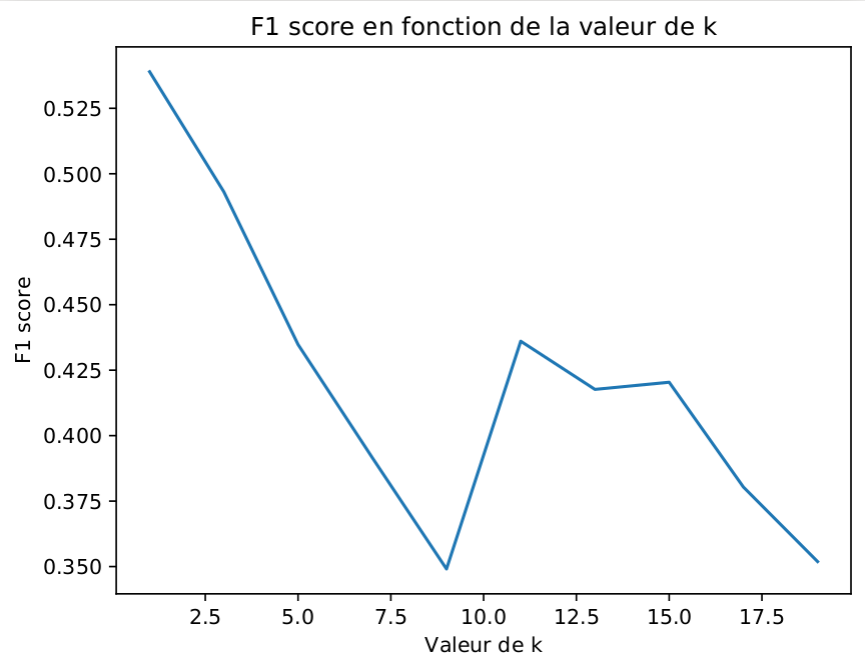
\includegraphics[width=\textwidth]{images/riemannKNN_valeur_de_k_brain_invader.png}
            \caption[]%
            {{\small Riemann knn  }}    
            \label{fig:mean and std of net24}
        \end{subfigure}
        \caption[ Visualisation des classes]
        {\small F1 Score(en cross validation) en fonction du nombre de voisin } 
        \label{fig:mean and std of nets}
    \end{figure*}
    


Sur la figure ci-dessous on peut voir que la valeur de K=1 est meilleur dans tous les cas : signaux brut, covariance sur les essais, et avec la géométrie de Riemann.
\section{Étude sur la longueur de la fenêtre optimale}
La longueur de la fenêtre c'est la durée utilisé pour découper un signal continu en plusieurs essais.
\begin{figure*}[h]
        \centering
        \begin{subfigure}[b]{0.475\textwidth}
            \centering
            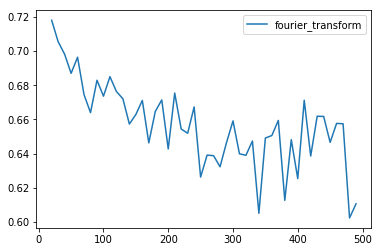
\includegraphics[width=\textwidth]{images/knn_tf_f1Score.png}
            \caption[Network2]%
            {{\small KNN transformée de fourier}}    
            \label{fig:mean and std of net14}
        \end{subfigure}
        \hfill
        \begin{subfigure}[b]{0.475\textwidth}  
            \centering 
            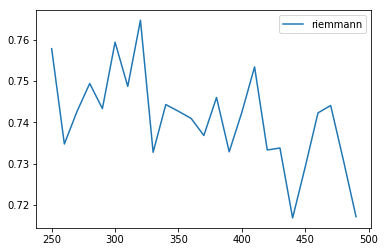
\includegraphics[width=\textwidth]{images/riemann_cov_knn_f1Score.png}
            \caption[]%
            {{\small Riemann Cov KNN }}    
            \label{fig:mean and std of net24}
        \end{subfigure}
        \vskip\baselineskip
        \begin{subfigure}[b]{0.475\textwidth}   
            \centering 
            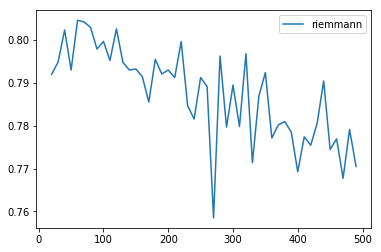
\includegraphics[width=\textwidth]{images/riemann_cov_MDM_f1Score.png}
            \caption[]%
            {{\small riemann MDM}}    
            \label{fig:mean and std of net34}
        \end{subfigure}
        \quad
        \begin{subfigure}[b]{0.475\textwidth}   
            \centering 
            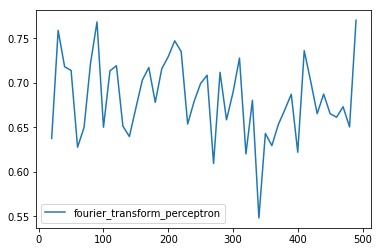
\includegraphics[width=\textwidth]{images/perceptron_tf_f1Score.png}
            \caption[]%
            {{\small SVM transformée de fourier }}    
            \label{fig:mean and std of net44}
        \end{subfigure}
        \caption[ F1 Score(en cross validation) en fonction du nombre de données par paquet]
        {\small F1 Score(en cross validation) en fonction du nombre de données dans la fenêtre temporelle} 
        \label{fig:mean and std of nets}
\end{figure*}
Les résultats sont obtenus avec une cross validation sur tous les participants mais en ne prenant en compte qu'un fichier par participant pour une question de mémoire vive.
F1-score des différents algorithmes sur brain invader : \\
\begin{table}[H]
\begin{tabular}{|l|l|l|l|l|}
\hline
nom de l'algorithme                                                              & 1 seconde         & 0,1 seconde       & 0,04 seconde      & moyenne           \\
\hline
passe bas KNN & 0,002487562189055 & \colorbox{gray!30}{0,126738794435858} & 0,004889975550122 & 0,044705444058345 \\
knn tf & 0,019002375296912 & 0,029919447640967 & \colorbox{gray!30}{0,124804992199688} & 0,057908938379189 \\
knn brut            & 0,071287128712871 & \colorbox{gray!30}{0,104810996563574} & 0,027681660899654 & 0,067926595392033 \\
SVM brut       & 0,181818181818182 & 0                 & \colorbox{gray!30}{0,214285714285714} & 0,132034632034632 \\
cov SVM & 0                 & 0,181818181818182 & \colorbox{gray!30}{0,235294117647059} & 0,13903743315508  \\
SVM tf & 0,125             & 0,125             & \colorbox{gray!30}{0,181818181818182} & 0,143939393939394 \\
passe bas SVM & 0,214285714285714 & 0,214285714285714 & \colorbox{gray!30}{0,235294117647059} & 0,221288515406162 \\
riemann MDM     & \colorbox{gray!30}{0,269889224572004} & 0,256206554121152 & 0,249661705006766 & 0,258585827899974\\
\hline
moyenne	& 0,110471273359342 &	0,129847461108181& 	\colorbox{gray!30}{0,159216308131781}\\
\hline
\end{tabular}
\captionof{table}{Résultat sur le dataset brain invader 1 participant}
\end{table}
On surligne en gris chaque meilleurs score par ligne.\\
Dans 3 des figures ci-dessus on remarque qu'avec des tailles de fenêtre très petites on a de très bons résultats. Cela vient du fait qu'on utilise des algorithmes tels que le KNN et le MDM et que, de plus, on est sur un seul participant. Donc on va juste chercher à faire correspondre les signaux qui sont proches temporellement et comme on modifie les labels par palier, cela donne de bon résultats de retrouver les voisins proches et prédire le même label. Je pense qu'on ne peut pas tirer assez d'information sur les corrélations des différents canaux pour faire du transfert, je n'ai malheureusement pas eu le temps de faire les tests.    

\section{Comparaison des différentes méthodes}
Tous les résultats suivant ont été obtenus avec les données d'un seul participant, avec une validation croisée en 5 parties.
\subsection{Tableau récapitulatif eye close/open}
Ci-dessous nous avons le tableau récapitulatif des F1-score en validation croisée en 5 parties sur les données d'un seul participant. On remarque que les approches de Riemann ont les meilleurs scores et ensuite le SVM avec transformée de Fourier.\\
\begin{center}
\begin{tabular}{|l|c|}
  \hline
  Nom de l'algorithme & f1-score\\
  \hline
  SVM sur les données brutes & 0.54 \\
  KNN sur les données brutes & 0.61\\
  Riemann Cov MDM  & 0.84 \\
  Riemann Cov KNN & 0.77\\
  SVM filtre passe bas & 0.60 \\
  KNN filtre passe bas & 0.59 \\
  SVM transformée de Fourier & 0.77 \\
  KNN transformée de Fourier & 0.72 \\
  \hline
\end{tabular}
\captionof{table}{Résultat sur le dataset eye close/open}
\end{center}
\subsection{Brain Invader}
Comme on peut le voir (ref : Table 1) tous les algorithmes ne sont pas présents, certains était trop longs à faire tourner et d'autre n'avaient pas encore été introduis et le seront pour le dataset DecMeg2014 qui suit. Peu de  prétraitement a été fait sur le signal(aucun filtre fréquentielle ni spatial) pour la géométrie de Riemann et cela change beaucoup les résultats juste un filtre passe bande peut améliorer les résultats comme on va le voir par la suite. C'est aussi pour cela qu'on retrouve un SVM en deuxième position. Il n'a pas été possible de comparer les résultats avec les résultats de l'auteur du dataset car il manquait la composition des groupes d'aliens qui clignotaient.\\
\subsection{DecMeg2014}

\paragraph{Méthodes d'évaluation}

Sur le dernier dataset DecMeg2014 nous disposons des données pour 16 participants, nous procéderons donc comme décrit ci-dessous pour l'évaluation de nos différentes méthodes :\\
Méthode 1 : entraînement sur une partie de 1 et eval sur 1 (validation croisée sur un seul)\\
Méthode 2 : entraînement sur 1 et évaluation sur tous les autres (16 expériences a faire)\\
Méthode 3 : entraînement sur 15 et évaluation sur 1 (16 expériences a faire )\\
Méthode 4 : entraînement sur 16 et eval sur 16 tout mélanger avec validation croisée.
\\
Ces façons d'évaluer nous permettent de tester plusieurs caractéristiques de nos modèles dont la capacité de transfert d'un participant à l'autre.
\\
Pour chaque test on sauvegardera le F1-score moyen sur les deux classes.
\\

\begin{table}[H]
\begin{center}
\begin{tabular}{|l|l|l|l|l|}
\hline
Nom de l’algorithme & Méthode 1         & Méthode 2           & Méthode 3          & Méthode 4          \\
\hline
CTR                 & 0,717 & 0.445 & 0.673 & 0.693 \\
conv1D              & 0,33         & - & 0.33               & 0.33               \\
passe bas SVM       & 0.33                & - & 0.33                  & 0.33                  \\
riemann MDM         & 0,5524            & -                & 0.43               & 0.535               \\
SVM brut            & 0.33                 & - & 0.33                  & 0.33                  \\
SVM TF              & 0.33                 & - & 0.33                  & 0.33      \\
\hline           
\end{tabular}
\end{center}
\end{table}
On a beaucoup de 0.33, cela correspond parfois au fait que le modèle prédit toujours la même classe. Mais parfois pour certain modèle ce n'est pas le cas, on a  0.53 pour la classe 1 et 0.13 pour la classe 2 par exemple pour le conv1D, je n'ai pas découvert pourquoi. \\
Grace à la méthode 3 on peut voir que les méthodes de Riemann sont les méthodes qui fonctionne le mieux pour le transfert et avec une marge significative. De plus cela montre la robustesse des méthodes de Riemann qui même avec un casque à électrodes placé différemment et un niveau de bruit élevé l'algorithme peut faire de bonne prédiction sur un nouveau participant.
\part{Conclusion}
D'après nos résultat nous pouvons conclure que d'une part les prétraitement sur le signal sont très important et que pour le moment avec des méthodes classiques de deep learning on n'arrive pas à faire mieux qu'avec des méthodes riemanniennes. Il pourrait être intéressant de combiner des méthodes de deep learning et de géométrie de Riemann.
\bibliographystyle{ieeetr}
\bibliography{MyLibrary} 


\end{document}
